\documentclass[tikz,border=5pt]{standalone}
\usepackage[UTF8]{ctex}
\usepackage{amsmath,amssymb}
\usetikzlibrary{arrows.meta,calc}
\tikzset{>=Stealth,line cap=round,line join=round,
 edge/.style={draw=black!75,thick},hidden/.style={black!40,dashed},
 dim/.style={black!60,<->},upforce/.style={blue!70!black,very thick,->},
 downforce/.style={red!70!black,very thick,->}}
\begin{document}
% 1. Parallel projection x=(1,0),y=(-.45,.32),z=(0,1).
% Water-frame instantaneous body: length l1, transverse w,h unchanged.
\begin{tikzpicture}[font=\small,x={(1cm,0cm)},y={(-.45cm,.32cm)},z={(0cm,1cm)}]
\fill[cyan!5](-1.4,-.2,-.6)--(6.7,-.2,-.6)--(6.7,-.2,3.35)--(-1.4,-.2,3.35)--cycle;
\draw[cyan!45!black,dashed](-1.4,-.2,3.35)--(6.7,-.2,3.35);
\node[above right]at(5.2,-.2,3.35){水面};
\draw[hidden](0,0,0)--(0,1.8,0)--(5,1.8,0);
\draw[hidden](0,1.8,0)--(0,1.8,1.4);
\filldraw[fill=gray!8,edge](0,0,0)--(5,0,0)--(5,0,1.4)--(0,0,1.4)--cycle;
\filldraw[fill=gray!16,edge](5,0,0)--(5,1.8,0)--(5,1.8,1.4)--(5,0,1.4)--cycle;
\filldraw[fill=blue!12,edge](0,0,1.4)--(5,0,1.4)--(5,1.8,1.4)--(0,1.8,1.4)--cycle;
\node at(2.8,.75,1.4){$A_1,\ p_t$};
\node at(2.45,0,.65){$V_1$};
\node[below]at(2.5,0,0){$p_b$};
\draw[dim](0,0,-.55)--(5,0,-.55)node[midway,below]{$l_1$};
\draw[dim](5.65,0,0)--(5.65,0,1.4)node[midway,right]{$h$};
\draw[dim](-.55,0,1.55)--(-.55,1.8,1.55)node[midway,above left]{$w$};
\draw[blue!70!black,thick,->](1.4,0,2.65)--(4.3,0,2.65)node[midway,above]{$v$};
\draw[->](-1.75,0,.1)--(-1.75,0,2.15)node[above]{$z$};
\draw[->](6.05,0,-.5)--(7.15,0,-.5)node[right]{$x$};
\end{tikzpicture}
% 2. Same prism in two frames; illustrated gamma=1.25 => 4:5 x length.
\begin{tikzpicture}[font=\small,x={(1cm,0cm)},y={(-.45cm,.32cm)},z={(0cm,1cm)}]
\foreach \dx/\len/\ar/\vol/\lab in{0/4/A_1/V_1/S,7.5/5/A_0/V_0/S'}{
 \begin{scope}[shift={(\dx,0,0)}]
 \draw[hidden](0,0,0)--(0,1.5,0)--(\len,1.5,0);
 \draw[hidden](0,1.5,0)--(0,1.5,1.4);
 \filldraw[fill=gray!8,edge](0,0,0)--(\len,0,0)--(\len,0,1.4)--(0,0,1.4)--cycle;
 \filldraw[fill=gray!16,edge](\len,0,0)--(\len,1.5,0)--(\len,1.5,1.4)--(\len,0,1.4)--cycle;
 \filldraw[fill=blue!10,edge](0,0,1.4)--(\len,0,1.4)--(\len,1.5,1.4)--(0,1.5,1.4)--cycle;
 \node at(.5*\len,.7,1.4){$\ar$};\node at(.5*\len,0,.6){$\vol$};
 \draw[dim](\len+.55,0,0)--(\len+.55,0,1.4)node[midway,right]{$h$};
 \node[above]at(.5*\len,0,2.9){$\lab$};
 \end{scope}
}
\draw[dim](0,0,-.55)--(4,0,-.55)node[midway,below]{$l_0/\gamma$};
\draw[dim](7.5,0,-.55)--(12.5,0,-.55)node[midway,below]{$l_0$};
\draw[blue!70!black,thick,->](1.2,0,2.25)--(3.2,0,2.25)node[midway,above]{$v$};
\node[below]at(2,0,-1.4){水静止，艇运动};
\draw[blue!70!black,thick,->](11.8,0,2.25)--(9,0,2.25)node[midway,above]{$-v$（水）};
\node[below]at(10,0,-1.4){艇静止，水运动};
\end{tikzpicture}
% 3. Vertical face forces applied to actual horizontal face centers.
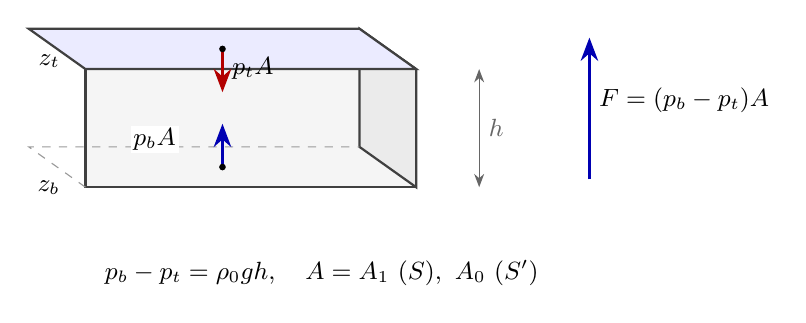
\begin{tikzpicture}[font=\small,x={(1cm,0cm)},y={(-.45cm,.32cm)},z={(0cm,1cm)}]
\filldraw[fill=gray!8,edge](0,0,0)--(4.2,0,0)--(4.2,0,1.5)--(0,0,1.5)--cycle;
\filldraw[fill=gray!16,edge](4.2,0,0)--(4.2,1.6,0)--(4.2,1.6,1.5)--(4.2,0,1.5)--cycle;
\filldraw[fill=blue!8,edge](0,0,1.5)--(4.2,0,1.5)--(4.2,1.6,1.5)--(0,1.6,1.5)--cycle;
\draw[hidden](0,0,0)--(0,1.6,0)--(4.2,1.6,0);
\draw[downforce](2.1,.8,1.5)--(2.1,.8,.95);
\node[right]at(2.1,.8,1.25){$p_tA$};
\draw[upforce](2.1,.8,0)--(2.1,.8,.55);
\node[left,fill=white,inner sep=1pt]at(1.55,.8,.35){$p_bA$};
\fill(2.1,.8,1.5)circle(1.2pt);\fill(2.1,.8,0)circle(1.2pt);
\draw[dim](5,0,0)--(5,0,1.5)node[midway,right]{$h$};
\node[left]at(-.2,0,1.6){$z_t$};\node[left]at(-.2,0,0){$z_b$};
\draw[upforce](6.4,0,.1)--(6.4,0,1.9);
\node[right]at(6.4,0,1.1){$F=(p_b-p_t)A$};
\node[below]at(3,0,-.8){$p_b-p_t=\rho_0gh,\quad A=A_1\ (S),\ A_0\ (S')$};
\end{tikzpicture}
% 4. beta=.6, l0=2.5, l1=2.0; x=.6ct and x=2+.6ct.
% Center worldline x=1+.6ct; P=(1.9,1.5),Q=(3.1,3.5).
\begin{tikzpicture}[font=\small]
\draw[->](-.5,0)--(5.3,0)node[right]{$x$};
\draw[->](0,-.3)--(0,5.1)node[above]{$ct$};
\draw[black!55,thick](0,0)--(2.88,4.8);
\draw[black!55,thick](2,0)--(4.88,4.8);
\node[above left]at(2.88,4.8){艇后端};
\node[above right]at(4.88,4.8){艇前端};
\draw[blue!65!black,thin,dotted](1,0)--(3.88,4.8);
\draw[blue!65!black,very thick,->](1.9,1.5)--(3.1,3.5);
\fill(1.9,1.5)circle(1.5pt);\node[right,fill=white,inner sep=1pt]at(1.9,1.5){$P$};
\fill(3.1,3.5)circle(1.5pt);\node[right,fill=white,inner sep=1pt]at(3.1,3.5){$Q$};
\node[blue!65!black,left,fill=white,inner sep=1pt]at(2.45,2.65){$\mathrm dx=v\,\mathrm dt$};
\draw[red!70!black,dashed](-.25,1)--(4.1,1)node[right]{$t=\mathrm{const}$};
\draw[green!45!black,dashed](-.25,-.05)--(4.9,3.04)node[right]{$t'=\mathrm{const}$};
\node[below,red!70!black,fill=white,inner sep=1pt]at(3.4,.95){水系等时};
\node[above left,green!45!black,fill=white,inner sep=1pt]at(4.75,2.95){艇系等时};
\node[below]at(2.6,-.55){$P,Q$ 位于同一艇体质心世界线};
\end{tikzpicture}
% 5. Definition diagram, not a fictional Euclidean direction of four-vectors.
\begin{tikzpicture}[font=\small]
\node[draw,rounded corners,align=center,minimum width=3.8cm,minimum height=1.2cm](A)at(0,0){水系 $S$\\$F_{1z}=\mathrm dp_z/\mathrm dt$};
\node[draw,rounded corners,align=center,minimum width=3.8cm,minimum height=1.2cm](B)at(7.5,0){艇系 $S'$\\$F_{2z}=\mathrm dp'_z/\mathrm dt'$};
\node[draw,rounded corners,align=center,minimum width=3.8cm,minimum height=1.2cm](C)at(0,-3){$f^z=\mathrm dp_z/\mathrm d\tau$\\$f^z=\gamma F_{1z}$};
\node[draw,rounded corners,align=center,minimum width=3.8cm,minimum height=1.2cm](D)at(7.5,-3){$f'^z=\mathrm dp'_z/\mathrm d\tau$\\$f'^z=F_{2z}$};
\draw[->,thick](A)--(B)node[midway,above,align=center]{$p'_z=p_z$\\$\mathrm dt'=\mathrm dt/\gamma$};
\draw[->,thick](A)--(C)node[midway,left]{$\mathrm dt/\mathrm d\tau=\gamma$};
\draw[->,thick](B)--(D)node[midway,right]{$\mathrm dt'/\mathrm d\tau=1$};
\draw[->,thick](C)--(D)node[midway,below]{$x$ 向变换：$f'^z=f^z$};
\end{tikzpicture}
% 6. Force curves, independent panels; no beta>=1 or plotting divergences.
\begin{tikzpicture}[font=\small]
\foreach \dx/\lab in{0/S,6.8/S'}{
 \begin{scope}[xshift=\dx cm]
 \draw[->](0,0)--(4.3,0)node[right]{$\beta$};
 \draw[->](0,0)--(0,3.5)node[above]{$F/K_0,\ G/K_0$};
 \foreach \b in{0,.3,.6,.9}{\draw(4.4*\b,.06)--(4.4*\b,-.06)node[below]{$\b$};}
 \foreach \y in{1,3,5}{\draw(.06,.6*\y)--(-.06,.6*\y)node[left]{$\y$};}
 \node at(2,3.85){$\lab$};
 \end{scope}
}
\draw[blue!70!black,thick]plot coordinates{(0.00000000,0.60000000) (0.04950000,0.59996203) (0.09900000,0.59984811) (0.14850000,0.59965818) (0.19800000,0.59939219) (0.24750000,0.59905003) (0.29700000,0.59863156) (0.34650000,0.59813664) (0.39600000,0.59756506) (0.44550000,0.59691661) (0.49500000,0.59619103) (0.54450000,0.59538806) (0.59400000,0.59450736) (0.64350000,0.59354860) (0.69300000,0.59251139) (0.74250000,0.59139533) (0.79200000,0.59019997) (0.84150000,0.58892481) (0.89100000,0.58756936) (0.94050000,0.58613304) (0.99000000,0.58461526) (1.03950000,0.58301538) (1.08900000,0.58133274) (1.13850000,0.57956659) (1.18800000,0.57771619) (1.23750000,0.57578072) (1.28700000,0.57375931) (1.33650000,0.57165106) (1.38600000,0.56945500) (1.43550000,0.56717011) (1.48500000,0.56479532) (1.53450000,0.56232947) (1.58400000,0.55977138) (1.63350000,0.55711977) (1.68300000,0.55437329) (1.73250000,0.55153054) (1.78200000,0.54859001) (1.83150000,0.54555012) (1.88100000,0.54240921) (1.93050000,0.53916550) (1.98000000,0.53581713) (2.02950000,0.53236213) (2.07900000,0.52879840) (2.12850000,0.52512374) (2.17800000,0.52133578) (2.22750000,0.51743206) (2.27700000,0.51340992) (2.32650000,0.50926657) (2.37600000,0.50499901) (2.42550000,0.50060407) (2.47500000,0.49607837) (2.52450000,0.49141829) (2.57400000,0.48661997) (2.62350000,0.48167929) (2.67300000,0.47659181) (2.72250000,0.47135277) (2.77200000,0.46595708) (2.82150000,0.46039922) (2.87100000,0.45467323) (2.92050000,0.44877270) (2.97000000,0.44269064) (3.01950000,0.43641945) (3.06900000,0.42995087) (3.11850000,0.42327584) (3.16800000,0.41638444) (3.21750000,0.40926573) (3.26700000,0.40190764) (3.31650000,0.39429676) (3.36600000,0.38641817) (3.41550000,0.37825512) (3.46500000,0.36978879) (3.51450000,0.36099784) (3.56400000,0.35185793) (3.61350000,0.34234111) (3.66300000,0.33241503) (3.71250000,0.32204183) (3.76200000,0.31117680) (3.81150000,0.29976647) (3.86100000,0.28774598) (3.91050000,0.27503534) (3.96000000,0.26153394)};
\draw[red!70!black,thick]plot coordinates{(0.00000000,0.60000000) (0.04950000,0.60003797) (0.09900000,0.60015193) (0.14850000,0.60034201) (0.19800000,0.60060842) (0.24750000,0.60095148) (0.29700000,0.60137156) (0.34650000,0.60186917) (0.39600000,0.60244486) (0.44550000,0.60309932) (0.49500000,0.60383330) (0.54450000,0.60464767) (0.59400000,0.60554339) (0.64350000,0.60652152) (0.69300000,0.60758325) (0.74250000,0.60872987) (0.79200000,0.60996276) (0.84150000,0.61128346) (0.89100000,0.61269363) (0.94050000,0.61419503) (0.99000000,0.61578961) (1.03950000,0.61747942) (1.08900000,0.61926669) (1.13850000,0.62115381) (1.18800000,0.62314334) (1.23750000,0.62523802) (1.28700000,0.62744080) (1.33650000,0.62975480) (1.38600000,0.63218340) (1.43550000,0.63473020) (1.48500000,0.63739905) (1.53450000,0.64019408) (1.58400000,0.64311969) (1.63350000,0.64618062) (1.68300000,0.64938193) (1.73250000,0.65272904) (1.78200000,0.65622777) (1.83150000,0.65988437) (1.88100000,0.66370555) (1.93050000,0.66769851) (1.98000000,0.67187101) (2.02950000,0.67623142) (2.07900000,0.68078874) (2.12850000,0.68555271) (2.17800000,0.69053384) (2.22750000,0.69574351) (2.27700000,0.70119408) (2.32650000,0.70689895) (2.37600000,0.71287268) (2.42550000,0.71913119) (2.47500000,0.72569179) (2.52450000,0.73257346) (2.57400000,0.73979700) (2.62350000,0.74738526) (2.67300000,0.75536338) (2.72250000,0.76375916) (2.77200000,0.77260335) (2.82150000,0.78193009) (2.87100000,0.79177742) (2.92050000,0.80218783) (2.97000000,0.81320898) (3.01950000,0.82489449) (3.06900000,0.83730497) (3.11850000,0.85050921) (3.16800000,0.86458563) (3.21750000,0.87962410) (3.26700000,0.89572819) (3.31650000,0.91301789) (3.36600000,0.93163322) (3.41550000,0.95173860) (3.46500000,0.97352870) (3.51450000,0.99723590) (3.56400000,1.02314023) (3.61350000,1.05158272) (3.66300000,1.08298353) (3.71250000,1.11786722) (3.76200000,1.15689859) (3.81150000,1.20093484) (3.86100000,1.25110348) (3.91050000,1.30892271) (3.96000000,1.37649440)};
\node[red!70!black,above left]at(3.96,1.38){$G_1/K_0=\gamma$};
\node[blue!70!black]at(2,-.65){$F_1/K_0=1/\gamma$};
\begin{scope}[xshift=6.8cm]
\draw[blue!70!black,thick](0,.6)--(3.96,.6);
\draw[red!70!black,thick]plot coordinates{(0.00000000,0.60000000) (0.04950000,0.60007595) (0.09900000,0.60030390) (0.14850000,0.60068422) (0.19800000,0.60121747) (0.24750000,0.60190446) (0.29700000,0.60274626) (0.34650000,0.60374416) (0.39600000,0.60489969) (0.44550000,0.60621465) (0.49500000,0.60769109) (0.54450000,0.60933134) (0.59400000,0.61113799) (0.64350000,0.61311393) (0.69300000,0.61526235) (0.74250000,0.61758675) (0.79200000,0.62009095) (0.84150000,0.62277912) (0.89100000,0.62565580) (0.94050000,0.62872590) (0.99000000,0.63199473) (1.03950000,0.63546805) (1.08900000,0.63915206) (1.13850000,0.64305343) (1.18800000,0.64717938) (1.23750000,0.65153765) (1.28700000,0.65613659) (1.33650000,0.66098518) (1.38600000,0.66609309) (1.43550000,0.67147071) (1.48500000,0.67712925) (1.53450000,0.68308077) (1.58400000,0.68933824) (1.63350000,0.69591566) (1.68300000,0.70282815) (1.73250000,0.71009200) (1.78200000,0.71772481) (1.83150000,0.72574564) (1.88100000,0.73417509) (1.93050000,0.74303549) (1.98000000,0.75235110) (2.02950000,0.76214823) (2.07900000,0.77245552) (2.12850000,0.78330420) (2.17800000,0.79472830) (2.22750000,0.80676506) (2.27700000,0.81945523) (2.32650000,0.83284353) (2.37600000,0.84697911) (2.42550000,0.86191610) (2.47500000,0.87771429) (2.52450000,0.89443980) (2.57400000,0.91216601) (2.62350000,0.93097454) (2.67300000,0.95095640) (2.72250000,0.97221343) (2.77200000,0.99485989) (2.82150000,1.01902444) (2.87100000,1.04485247) (2.92050000,1.07250886) (2.97000000,1.10218140) (3.01950000,1.13408486) (3.06900000,1.16846602) (3.11850000,1.20560985) (3.16800000,1.24584718) (3.21750000,1.28956427) (3.26700000,1.33721497) (3.31650000,1.38933612) (3.36600000,1.44656742) (3.41550000,1.50967727) (3.46500000,1.57959687) (3.51450000,1.65746572) (3.56400000,1.74469322) (3.61350000,1.84304371) (3.66300000,1.95475555) (3.71250000,2.08271186) (3.76200000,2.23069058) (3.81150000,2.40374082) (3.86100000,2.60876654) (3.91050000,2.85546442) (3.96000000,3.15789474)};
\node[red!70!black,left]at(3.9,2.8){$G_2/K_0=\gamma^2$};
\node[blue!70!black]at(2,-.65){$F_2/K_0=1$};
\end{scope}
\node[below]at(5.2,-1.25){$K_0=\rho_0V_0g$；两图的 $\beta$ 为同一相对速度};
\end{tikzpicture}
\end{document}
